\documentclass{article}
\author{Junseo Shin \& Brendan Mayo}
\date{}
\title{Lab Notebook: Noise Fundamentals}

\usepackage{custom}
% use myrefs.bib for bibliography
\begin{document}

\maketitle
\tableofcontents
\pagebreak


\pagestyle{fancy}
\lhead{Junseo Shin \& Brendan Mayo}
\rhead{Lab Notebook: Noise Fundamentals}
\chead{11/5/24}
% Day 1

\section*{Intro}
\addcontentsline{toc}{section}{Intro}

\begin{itemize}
    \item John noise `mean square' voltage
    \begin{align*}
        \langle V_J^2 (t) \rangle = 4k_B TR\Delta f
    \end{align*}
    where $k_B$ is Boltzmann's constant, $T$ is temperature, $R$ is resistance, and $\Delta f$ is the bandwidth;
    \item Bandwidth $\Delta f$ is the range of frequencies tha we arrange to be sensitive to the `noise'source'
    \item e.g. $T = 295$ K, $ k_B = \qty{1.38e-23}{J/K} $, $\Delta f = \qty{e5}{Hz}$, $R = \qty{e5}{\ohm}$
    \begin{align*}
        \langle V_J^2 (t)\rangle = 4 \times \qty{1.38e-23}{J/K} \times \qty{295}{K} \times \qty{1e5}{Hz} \times \qty{1}{\Omega} = \qty{1.3e-17}{V^2} = \qty{1.63e-10}{V^2}
    \end{align*}
\end{itemize}
\section*{Day One}
Today we focused on reading through the manual and had time to work through sections 0 and most of 1. We successfully collected data and we were able to calculate Johnson noise.
\begin{figure}[h]
    \centering
    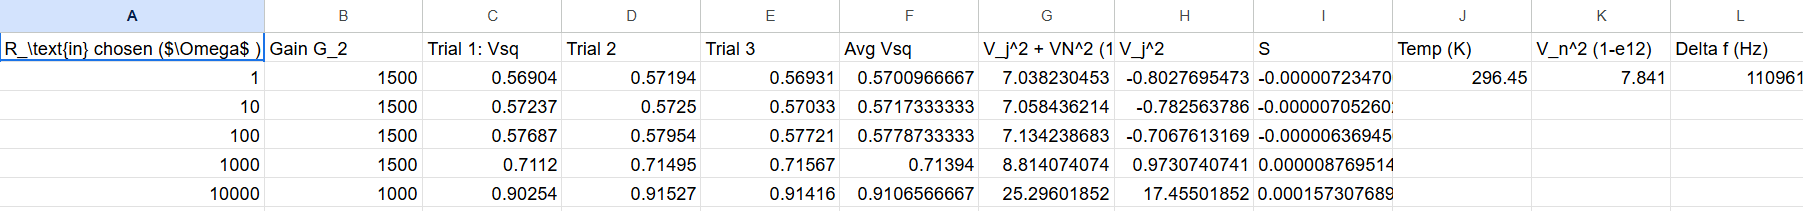
\includegraphics[width=0.8\textwidth]{lab_notebook/day1.PNG}
   
    \label{Section 1 data}
\end{figure}
\section*{Day Two}
Today we worked through the remainder of section 1 and all of section 2. We collected data and studied Johnson noise and its dependence on both resistance and bandwidth. We were able to calculate a Boltzman constant that was somewhat accurate. In section 2 we experimented with various band-pass filters and successfully saw a bandwidth. We then had some time left to begin reading section 7. 
\begin{figure}[h]
    \centering
    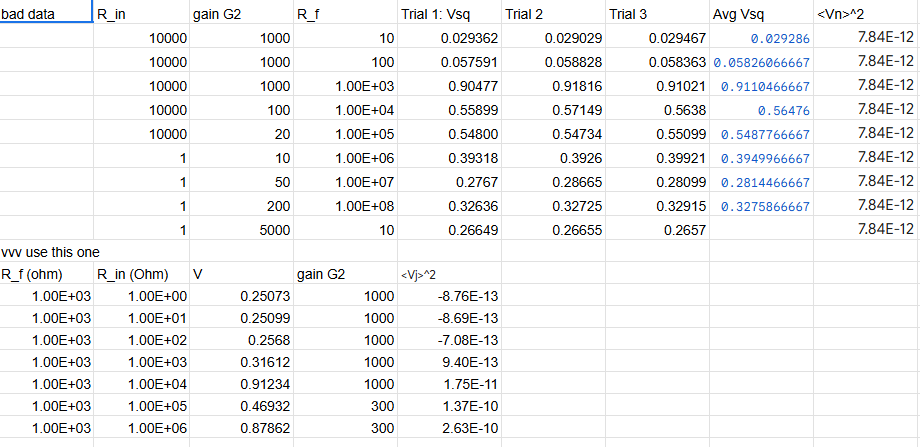
\includegraphics[width=0.8\textwidth]{lab_notebook/day2.PNG}
   
    \label{Section 1 data}
\end{figure}
\begin{figure}[h]
    \centering
    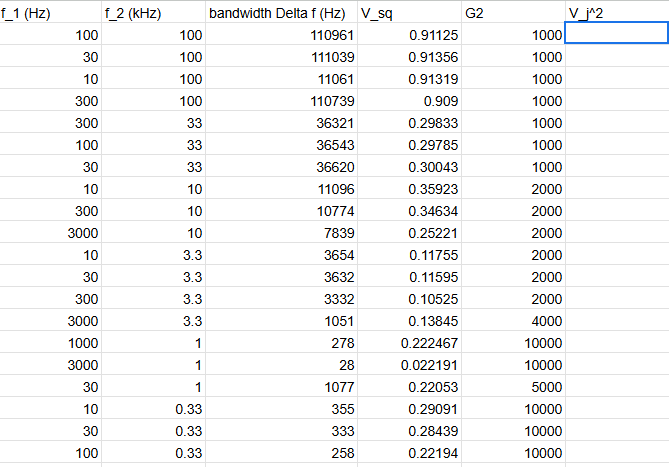
\includegraphics[width=0.8\textwidth]{lab_notebook/day2-2.PNG}
   
    \label{Section 1 data}
\end{figure}
\section*{Day Three}
Today we completed section 7. We successfully collected data and calculated noise density at various resistances, bandwidths, and voltages. We compared the calculated data to the manual and found that our results were accurate. We then read through section 4 and began to collect data on the relationship between temperature and the Johnson noise temperature. W successfully cooled with LN2 and recorded measurements of new voltages at various gains and resistances.
\begin{figure}[h]
    \centering
    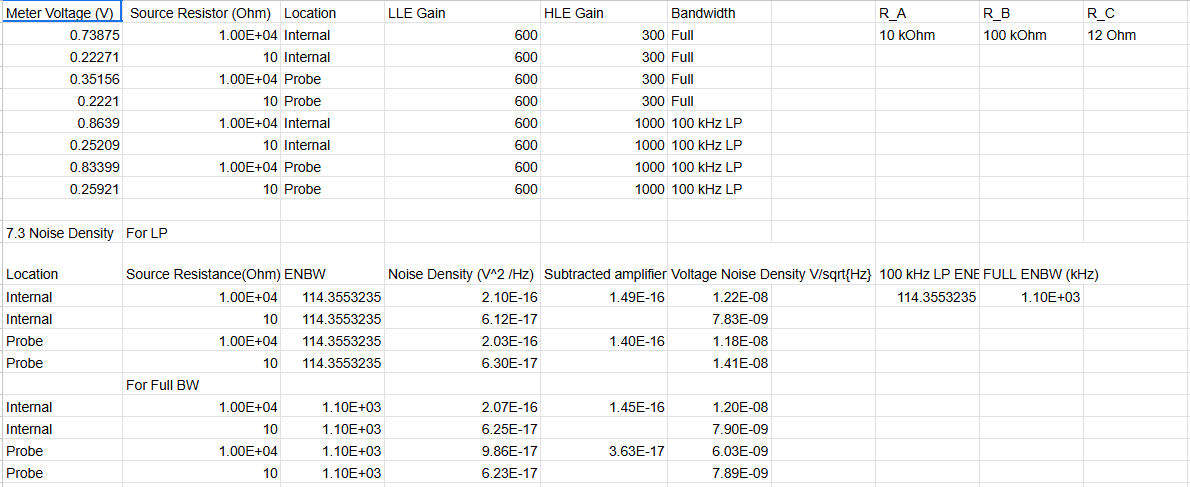
\includegraphics[width=0.8\textwidth]{lab_notebook/day3.PNG}
   
    \label{Section 1 data}
\end{figure}
\begin{figure}[h]
    \centering
    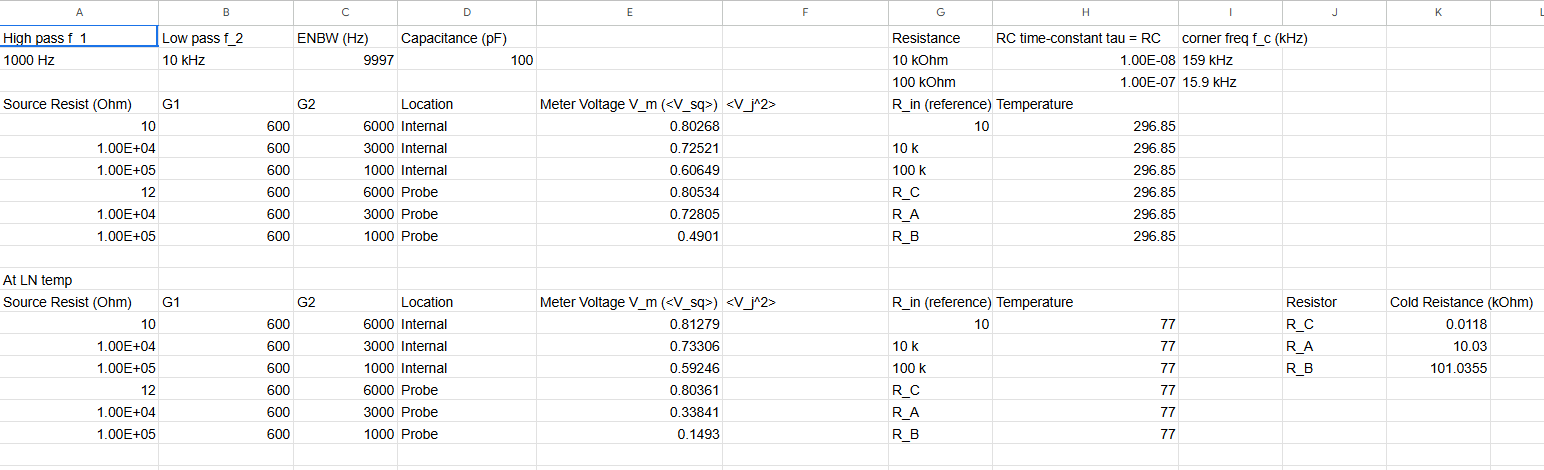
\includegraphics[width=0.8\textwidth]{lab_notebook/day3-2.PNG}
   
    \label{Section 1 data}
\end{figure}
\section*{Day Four}
Today we focused on analyzing the data in the sheets and differentiating between accurate and inaccurate data. We also started a Jupiter notebook in order to graph our Johnson noise vs temperature, resistance, and bandwidth.  
\section*{Day Five}
Today we continued working on the graphs and making them look the best we could. We also created a graph of what an ideal bandwidth should look like so now we are able to compare the bandwidth we measured to the theoretical one. At the very end of today, we started to discuss what our presentations should look like and we decided that Brendan would be doing his presentation on what Johnson noise is and explaining its dependencies as well as applications, and Junseo's presentation would discuss our results that we collected in the experiment and discuss our conclusions. 
\begin{figure}[h]
    \centering
    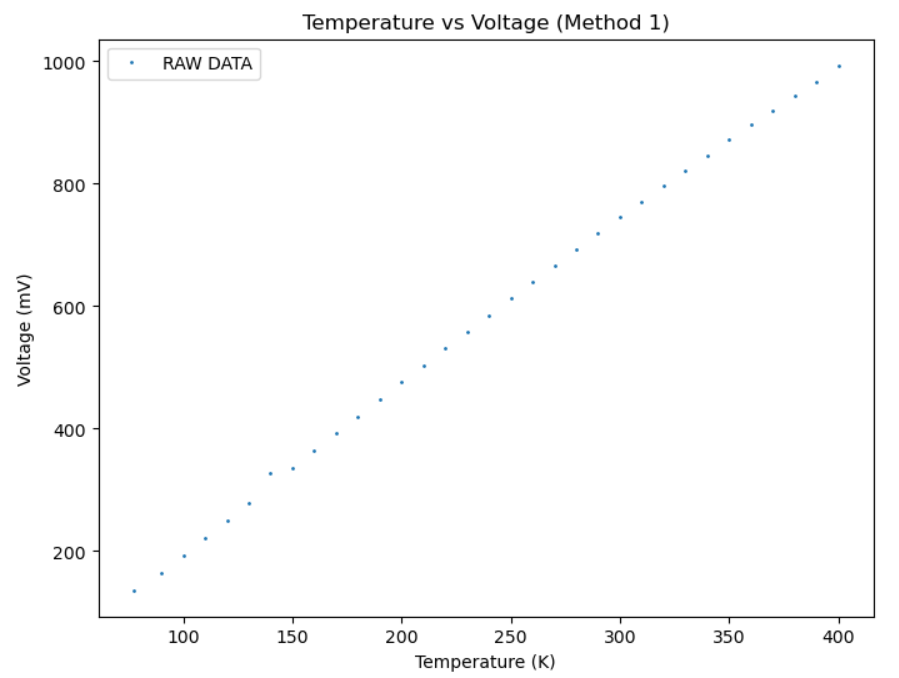
\includegraphics[width=0.8\textwidth]{lab_notebook/tempvsNoise.PNG}
   
    \label{Section 1 data}
\end{figure}
\begin{figure}[h]
    \centering
    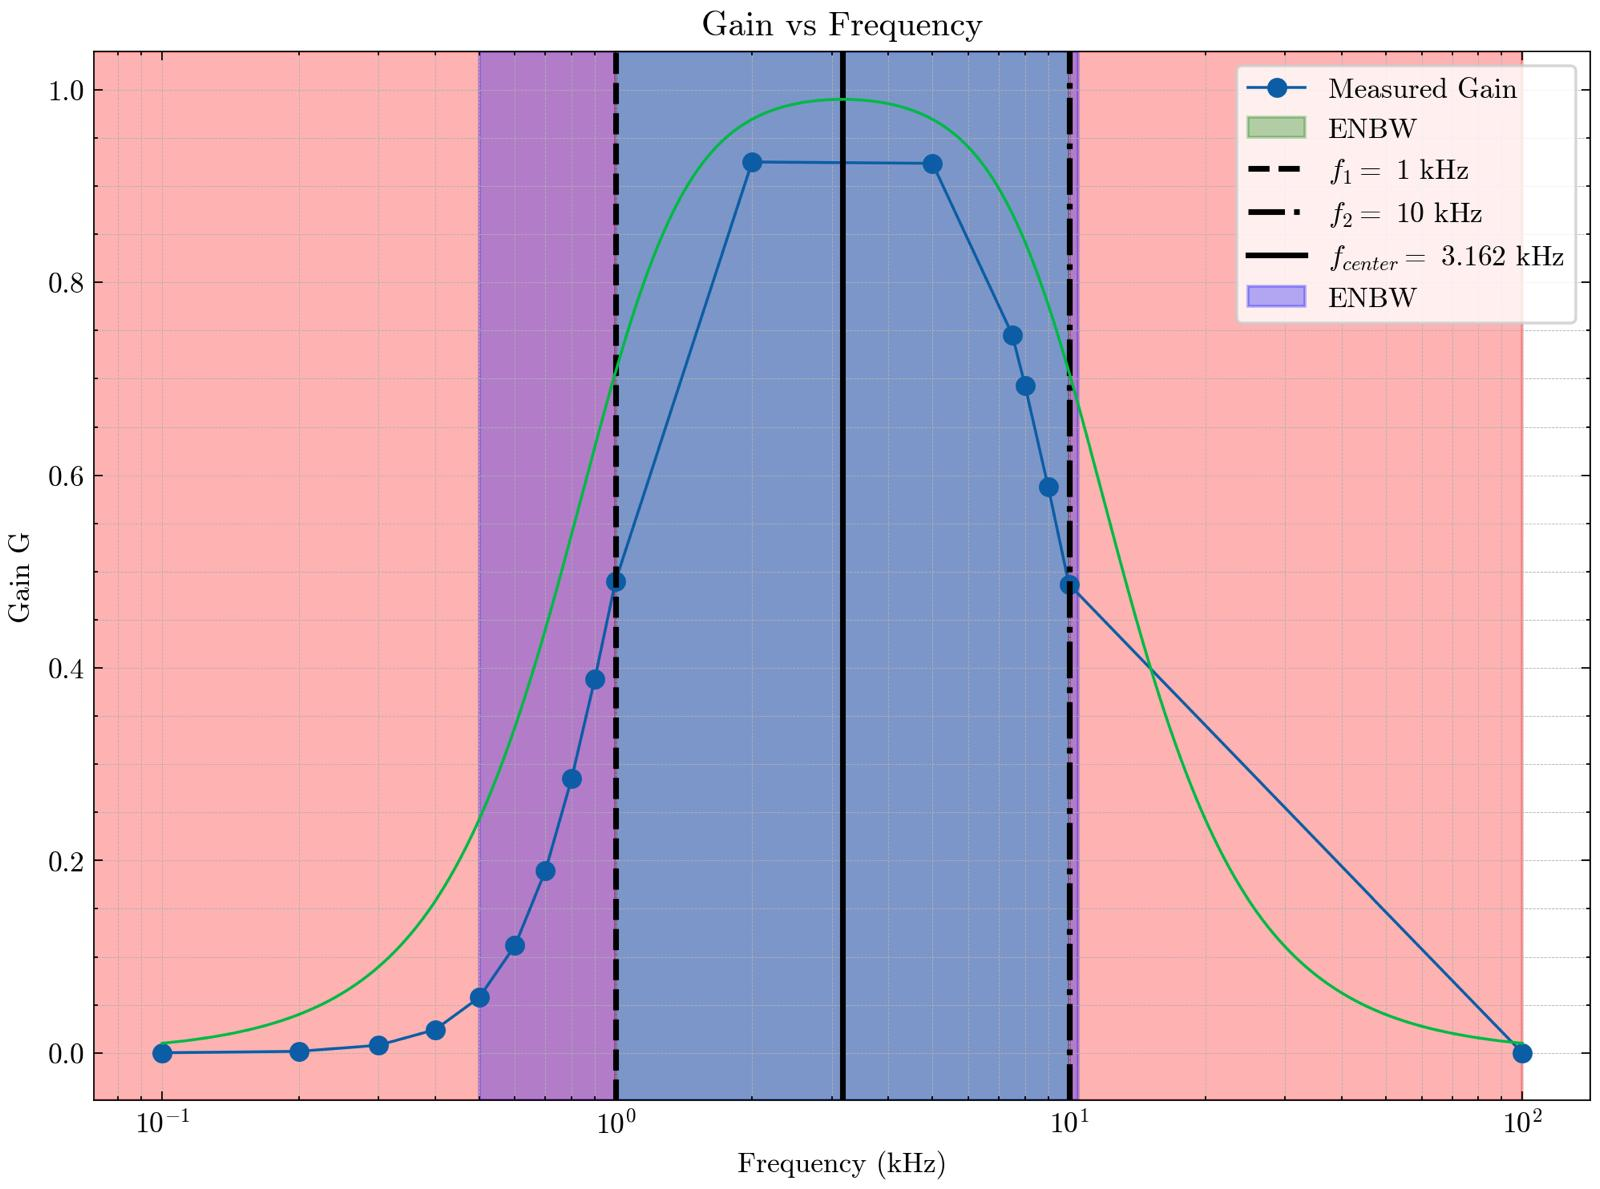
\includegraphics[width=0.8\textwidth]{lab_notebook/gain vs frequency.jpg}
   
    \label{Section 1 data}
\end{figure}
\section*{Day Six}
Today we primarily worked separately to create outlines and slides for our presentations. 
\bibliography{myrefs}
\bibliographystyle{plain}
\nocite{PhysRev.21.483}
\end{document}